\documentclass[../main.tex]{subfiles}
\begin{document}

\subsection{Szyfrowanie, podpis elektroniczny}


\subsubsection{Szyfrowanie z kluczem}
\begin{itemize}
    \item liczba lub kilka liczb, składająca się z kilkudziesięciu do kilku tysięcy bitów
    \item służy do szyfrowania i odszyfrowywania rzeczy
    \item teoretycznie możliwy do złamania brute forcem (w praktyce niezbyt)
    \item różne algorytmy szyfrowania
    \begin{itemize}
        \item Szyfrowanie z kluczem symetrycznym\\
        Szyfrowanie dużych porcji danych przy użyciu jednego klucza ułatwia złamanie
        szyfru. Dlatego klucz symetryczny powinien być zmieniany. Może być przesłany zaszyfrowany przy pomocy techniki z kluczem
        publicznym i prywatnym. Można generować oddzielne klucze sesji i szyfrować je
        wcześniej uzgodnionym tajnym kluczem symetrycznym. Klucze symetryczne mogą być też
        zmieniane co określony czas lub co określoną liczbę bajtów, z użyciem specjalnych
        protokołów.
        \begin{itemize}
            \item Data Encryption Standard DES, 3DES
            \item RC - szyfr strumieniowy wykorzystywany w szyfrowaniu ramek w sieciach bezprzewodowych WiFi/WPA
            \item Advanced Encryption Standard AES - szyfr blokowy, np WPA2
        \end{itemize}
        \item Szyfrowanie z kluczem asymetrycznym
        \begin{itemize}
            \item Szyfrowanie i odszyfrowanie jest tu realizowane przy pomocy pary kluczy - prywatnym
            (tajnym) i publiczny (znany). Jeden szyfruje, drugi odszyfrowywuje.
            \item Odgadnięcię jednego z kluczy praktycznie niemożliwe nawet przy znajomości drugiego
            \item Szyfrujemy coś czyimś kluczem publicznym, by tylko ten ktoś mógł to odszyfrować (swoim kluczem prywatnym)
            \item wielokrotnie kosztowniejsze
            czasowo od szyfrowania z kluczem symetrycznym
            \item używane do uzgodnienia kluczy symetrycznych
            \item algorytm RSA
        \end{itemize}
    \end{itemize}

\end{itemize}

\subsubsection{Skrót (hash)}
\begin{itemize}
    \item skrót wiadomości w podpisach cyfrowych, tworzony za pomocą funkcji haszujacej
    \item 128 bitów (MD5), 160 bitów(SHA-1), 224-512 bitów (rodzina SHA-2)
    \item jeśli w oryginalnej wiadomości (pliku)
    zmieniony zostanie chociaż jeden bit, to skrót będzie zupełnie inny niż ten, który został
    utworzony przed zmianą.
    \item  Algorytmy haszujące są deterministyczne,
    \item odtworzenie oryginalnej wiadomości ze skrótu jest prawie niemożliwe
\end{itemize}



\subsubsection{Podpis cyfrowy}
\begin{itemize}
    \item Zaszyfrowanie kluczem prywatnym daje gwarancję, że zaszyfrowana wiadomość pochodzi z
    odpowiedniego źródła
    \item Samej podpisywanej wiadomości nie musi się szyfrować. Generowany jest jej skrót
    i ten skrót szyfrowany jest z wykorzystaniem klucza
    prywatnego osoby podpisującej. Zaszyfrowany skrót stanowi podpis cyfrowy. Niezaszyfrowana wiadomość może być przesłana jawnie razem z zaszyfrowanym skrótem
    (czyli podpisem cyfrowym).
    \item Odbiorca odszyfrowuje skrót używając klucza
    publicznego nadawcy. Potem tworzy skrót wiadomości używając tej samej funkcji haszującej. Jeśli wyniki
    obu operacji są identyczne, to znaczy, że wiadomość na pewno
    podpisał określony nadawca, a ponadto nikt po tej wiadomości nie zmienił już po podpisaniu.
    \item Po podpisaniu dodatkowo możemy wiadomość zaszyfrować, ale to nie
    należy już do samego podpisu.
\end{itemize}

\subsubsection{Klucze publiczne i prywatne, infrastruktura kluczy publicznych}
\begin{itemize}
    \item Klucze mogą być generowane na komputerze
    lokalnym przy pomocy odpowiedniego oprogramowania i powinny być podpisane przez
    jakieś centrum certyfikacyjne.
    \item Centrum certyfikacyjne (CA) wydaje tzw. certyfikaty cyfrowe zawierające m.in:
    \begin{itemize}
        \item Identyfikator osoby/firmy/obiektu
        \item Identyfikator CA, który wydał certyfikat
        \item Numer identyfikacyjny certyfikatu
        \item Cel stosowania (np. podpisywanie bezpiecznych stron WWW albo podpisywanie listów elektronicznych)
        \item Wartość klucza publicznego
        \item Okres ważności
        \item Podpis cyfrowy wydawcy
    \end{itemize}
    \item Jeśli ufamy danemu CA, to ufamy, że zawarty w certyfikacie klucz publiczny jest rzeczywiście prawdziwy.
    W systemach operacyjnych oraz różnych programach
    jest wpisana lista zaufanych CA.
    Zarządzanie centrum certyfikacyjnym jest realizowane na przez konsolę MMC.
    \item Niezależnym standardem opisującym tworzenie kluczy, rejestrowanie i wykorzystywanie
    certyfikatów jest PGP (Pretty Good Privacy). Powstał standard Open PGP.

\end{itemize}

\subsubsection{Bezpieczne protokoły: IPSec, SSL, TLS}

Bezpieczne protokoły powinny zapewniać:
\begin{itemize}
    \item Poufność przesyłanych danych (osoby niepowołane nie powinny móc odczytać danych).
    \item Autentyczność (dane pochodzą rzeczywiście od określonego źródła).
    \item Integralność (nikt danych nie zmienił).
\end{itemize}

Bezpieczne protokoły mogą być wykorzystywane:
\begin{itemize}
    \item w warstwie aplikacji- szyfrowanie komunikatów HTTPS, protokoły SSL, TLS,
    \item między warstwą sieci a transportu- szyfrowanie
    pakietów IP – protokół IPSec,
    \item w warstwie łącza danych - szyfrowanie ramek, np. WEP,
    WPA, WPA2 w sieciach bezprzewodowych.
\end{itemize}


Protokoły szyfrujące przesyłane dane
\begin{itemize}
    \item SSL (warstwa aplikacji) – Używany do zabezpieczania innych protokołów, wykorzystuje
    połączenie szyfrowania asymetrycznego z kluczem publicznym i symetrycznego. Często
    wykorzystywany z HTTP w sieci WWW (HTTPS).
    \item TLS (warstwa aplikacji) – Podobny do SSL.
    \item SMB - Server Message Block Signing, znany też jako Common Internet File System CIFS) – do
    transferu plików, umieszcza cyfrowe podpisy w każdym bloku danych.
    \item S/MIME – Secure Multpurpose Internet Mail Extensions – szyfruje i umieszcza podpisy
    cyfrowe w wiadomościach pocztowych e-mail. Jest rozszerzeniem MIME, standardu
    włączania danych binarnych do listów elektronicznych.
    \item IPSec (warstwa IP)
\end{itemize}

\subsubsection{Protokół IPSec}
\begin{itemize}
    \item warstwa IP
    \item może szyfrować dane pochodzące z dowolnej
    aplikacji, proces szyfrowania i deszyfrowania jest niewidoczny dla użytkownika
    \item framework umożliwiający wykorzystanie pewnych protokołów (Authentication Headers AH i Encapsulating Security Payloads ESP)i
    metod według określonych zasad.
\end{itemize}



Cechy IPSec:
\begin{itemize}
    \item Autentyczność i integralność danych.\\
    AH umożliwia sprawdzenie autentyczności komputerów uczestniczących
    w transmisji, umożliwia też sprawdzenie integralności danych. Nagłówek IP oraz dane są
    zabezpieczone przed modyfikacją.
    \item Szyfrowanie danych.\\
    ESP zapewnia szyfrowanie danych oraz autentyczność i integralność danych. ESP może być
    używany samodzielnie lub z AH.
\end{itemize}

Przed przesyłaniem danych strony komunikujące się uzgadniają szczegóły takie jak sposób
uwierzytelniania, wymiana kluczy, algorytmy szyfrowania.
Polityki stosowania IPSec – w systemach Microsoft Windows ustala się politykę (zasadę,
policy) kiedy IPSec ma być automatycznie zastosowany. W wersji Windows XP były trzy
predefiniowane polityki:
\begin{itemize}
    \item Client (respond only) - transmisje bez IPSec, chyba że druga strona zażąda IPSec
    \item Server (request security) - żądanie transmisji IPSec, ale jeśli druga strona nie
    implementuje IPSec, to komunikacja bez IPSec
    \item Secure server (require security) - żądanie transmisji IPSec, jeśli druga strona nie
    implementuje IPSec, to komunikacja nie jest kontynuowana.
\end{itemize}


Tryby działania IPSec (zarówno AH jak i ESP):
\begin{itemize}
    \item Tryb transportu (w sieci lokalnej) między dwoma punktami końcowymi transmisji.
    \item Tryb tunelowania – szyfrowanie w niezabezpieczonej części sieci (np. dane między
    biurami przesyłane przez Internet).
\end{itemize}

Metody uwierzytelniania w IPSec:
\begin{itemize}
    \item Kerberos,
    \item Oparty o certyfikaty cyfrowe,
    \item Klucz dzielony (przechowywany we właściwościach napis jednakowy dla obu
    komunikujących się stron).
\end{itemize}

\textbf{Filtry IPSec}\\
Filtr IPSec pozwala na automatyczne przepuszczenie datagramów IP, blokowanie lub użycie
negocjacji (i w konsekwencji użycie IPSec) w zależności od źródła i miejsca docelowego IP,
protokołu transportowego, portów źródłowych i docelowych.


\subsubsection{SSL - Secure Socket Layer}
\begin{itemize}
    \item jego zadaniem jest zabezpieczanie informacji przesyłanych siecią.
    \item wykorzystywany przy przesyłaniu np. danych osobistych, numerów kart kredytowych.
    \item często prezentowany jako protokół, który leży
    powyżej warstwy transportu (TCP, UDP) i sieci (IP) a poniżej warstwy aplikacji (np. HTTP, FTP,
    SMTP, TELNET)
    \item W modelu ISO OSI jest przypisany do warstwy prezentacji (zatem do
    warstwy aplikacji w modelu TCP/IP)
    \item jest protokołem otwartym
    \item wykorzystuje szyfrowanie symetryczne z kluczem publicznym
    \item protokoły zabezpieczone SSL oznaczane są jako HTTPS (dla HTTP), FTPS (dla FTP) itd.
\end{itemize}

\begin{figure}[H]
    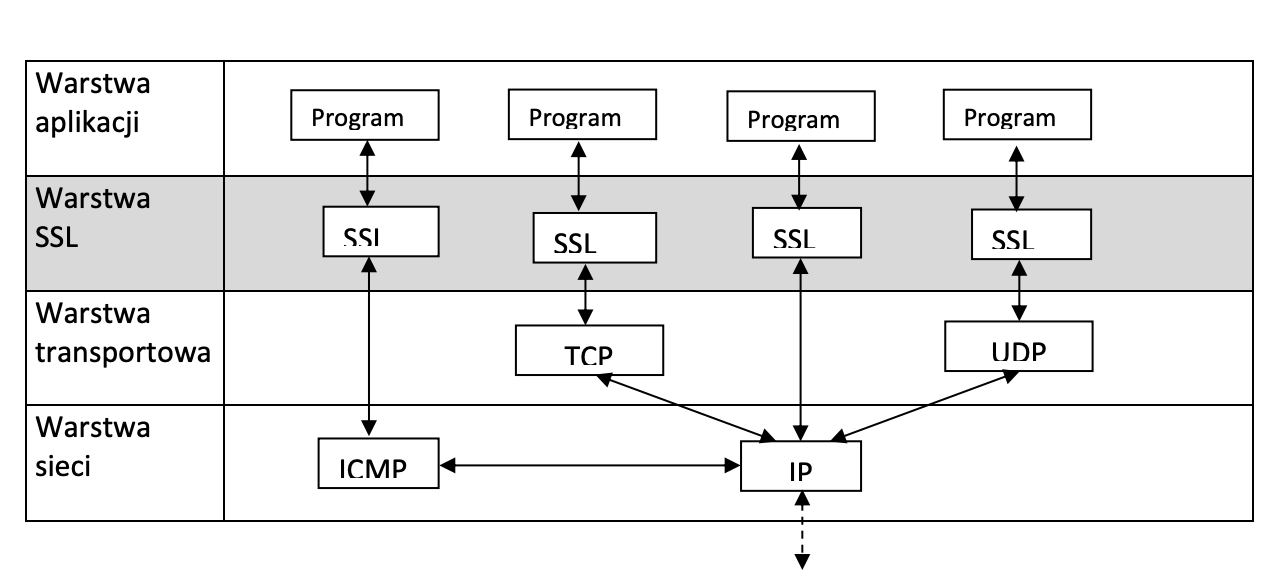
\includegraphics[width=\linewidth]{ssl.png}
\end{figure}

Podstawowe cechy protokołu SSL:
\begin{itemize}
    \item Zapewnia autoryzację serwerów internetowych i (opcjonalnie) klientów (utrudnia
    podszywanie pod autoryzowanych usługodawców i użytkowników)
    \item Zapewnia szyfrowanie - poufność przesyłanych informacji.
    \item Stosuje sumy kontrolne dla zapewnienia integralności danych.
\end{itemize}

Po nawiązaniu połączenia następuje wymiana informacji (certyfikatów CA i kluczy publicznych)
uwierzytelniających serwera i (opcjonalnie) klienta.
Serwer i klient uzgadniają również algorytmy szyfrowania –
najsilniejsze dostępne jednocześnie obu stronom.
Następnie serwer i klient generują klucze sesji (symetryczne), które są szyfrowane kluczem
publicznym drugiej strony. Klucze sesji są odszyfrowywane przy pomocy klucza prywatnego i
następnie służą do szyfrowania danych.


Numery portów przy włączeniu SSL:

\begin{tabular}{|c|c|c|}
    \hline
    Protokół & Port standardowy & Port SSL\\
    \hline
    HTTP & 80 & 443\\
    \hline
    IMAP4 & 143 & 993\\
    \hline
    POP3 & 110 & 995\\
    \hline
\end{tabular}


\end{document}